\chapter{Testování}
\label{chap:testovani}

Testování výsledné aplikace probíhalo na sestavě Intel\textregistered Core\texttrademark i7 CPU         950, frekvence 3.07GHz, 8 logických jader, 12288 MB RAM, GeForce GTX 470/PCI/SSE2. Rozlišení obrazu bylo pro všechny testy fixováno na 1280$\times$720px. Veškeré naměřené hodnoty fps (resp. zobrazovacích časů), jsou brány jako minimum dané veličiny za určitou dobu (typicky 10-20 vteřin). Měření těchto hodnot bylo prováděno pomocí tzv. TIMER\_QUERY. Jde o mechanismus, který měří čas potřebný pro vykreslení přímo na GPU pomocí Query Object asynchroního dotazu. Hodnota je určována s přesností na nanosekundy, ale uváděné hodnoty (v ms) jsou pro přehlednost zaokrouhleny na menší počet desetinných míst.


%%%%%%%%%%%%%%%%%%%%%%%%%%%%%%%%%%%%%
%	LOD0 vs LOD1
%
\begin{figure}[!hbt]
\begin{center}
$\begin{array}{ccc}
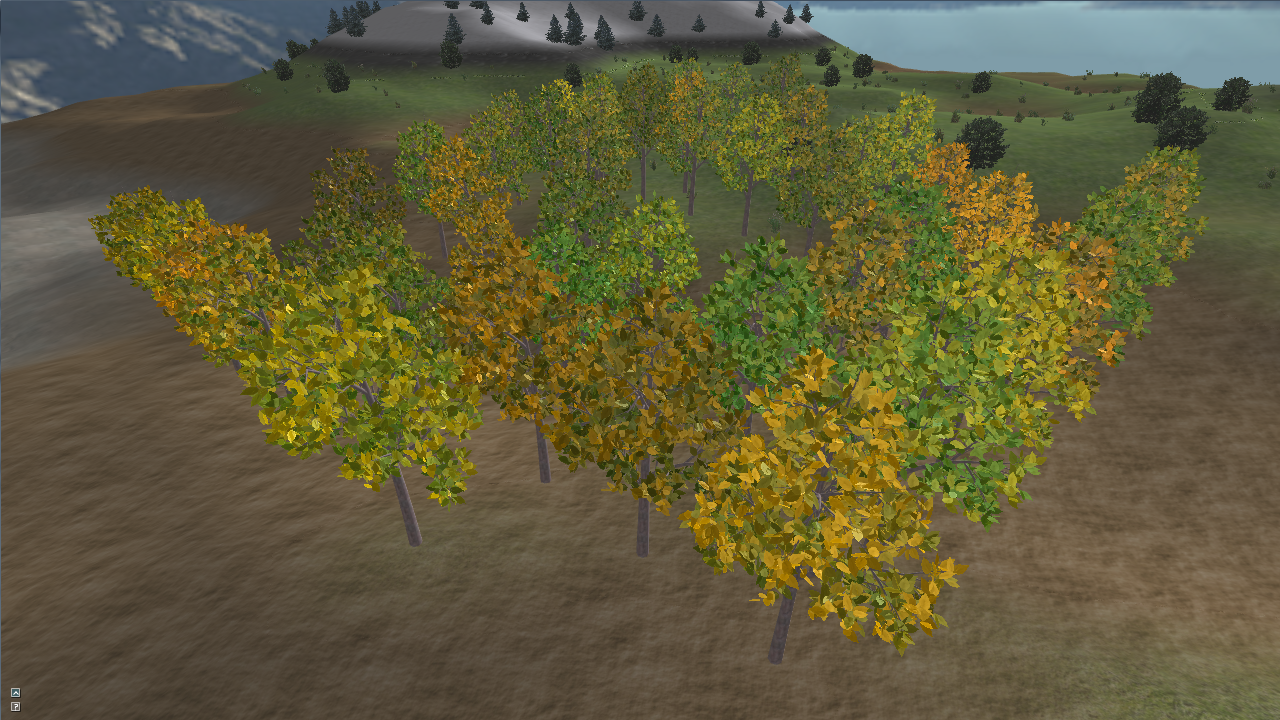
\includegraphics[width=0.3\textwidth]{./testing/LOD0only50.png}&
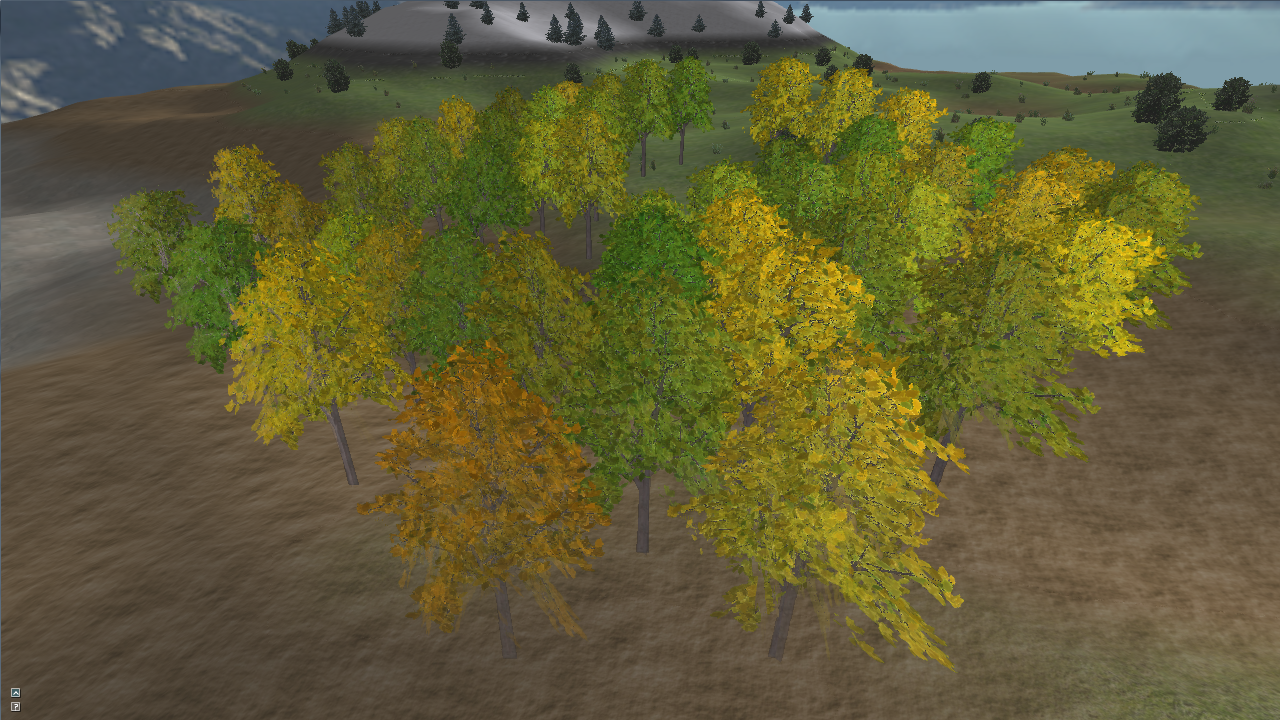
\includegraphics[width=0.3\textwidth]{./testing/LOD1only50.png}&
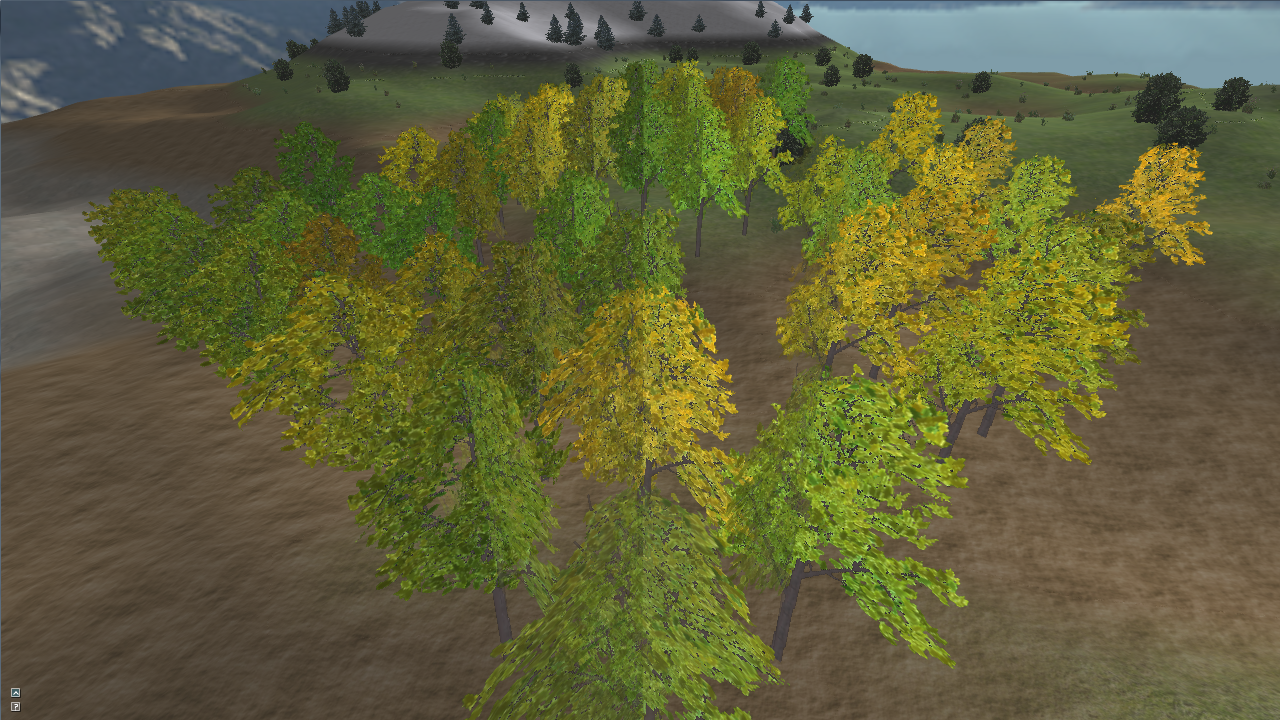
\includegraphics[width=0.3\textwidth]{./testing/LOD2only50.png}
\\
(a)&(b)&(c)
\end{array}$
\end{center}
\caption[Náhledy testovací scény]%
{Náhledy z testování, scéna SMALL FOREST s 50 instancemi, (a) LOD0,  (b) LOD1, (c) LOD2, 0\label{fig:testONLYsmall}
}
\end{figure}

Nejprve byla testována kvalita a rychlost zobrazování různých úrovní LOD. Pro tyto účely byly fixovány dvě scény s různým počtem instancí stromů. Scéna {\bf SMALL FOREST} představuje pohled na menší les (max. 50 instancí). Všechny instance by se měly nacházet v pohledovém prostoru kamery. Podobu scény při zobrazení všech stromů pouze v určitém LOD zachycují obrázky~\ref{fig:testONLYsmall}

\pagebreak
Pro testování rozsáhlejších porostů (až 1000 instancí) byla používána scéna {\bf FOREST} (viz obr.~\ref{fig:testONLY}).
\begin{figure}[!hbt]
\begin{center}
$\begin{array}{ccc}
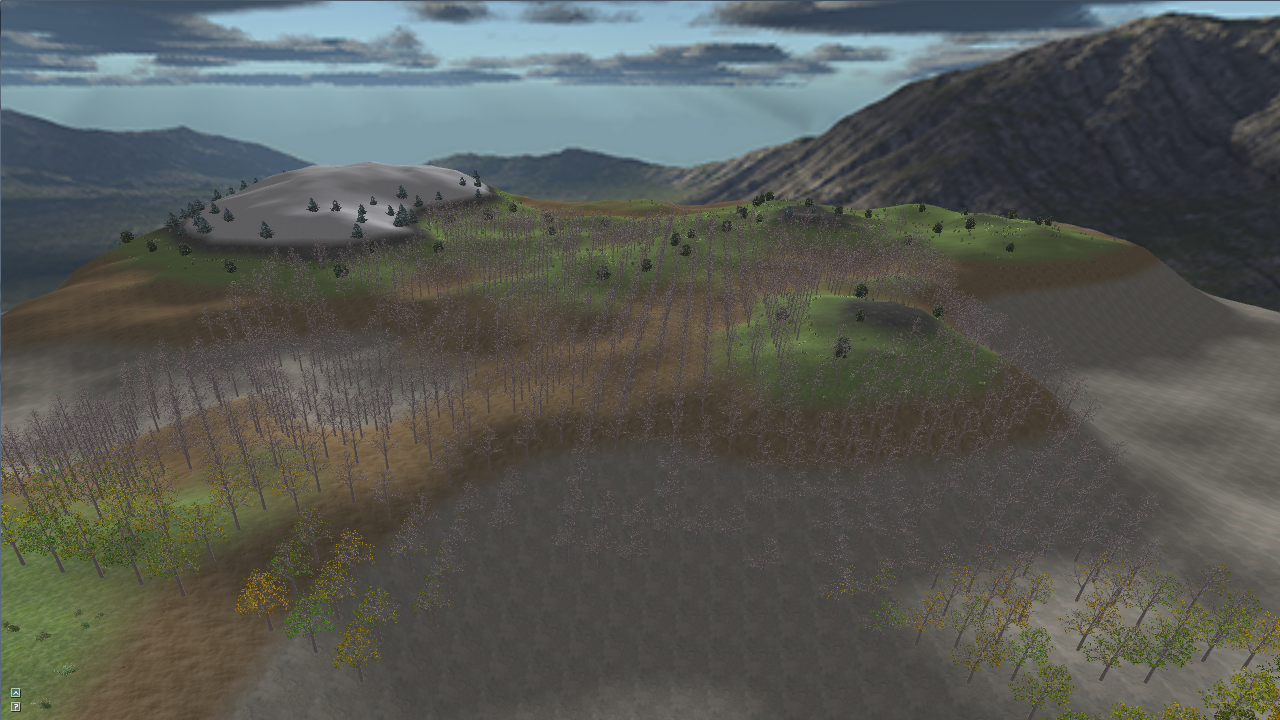
\includegraphics[width=0.3\textwidth]{./testing/LOD0only1000.png}&
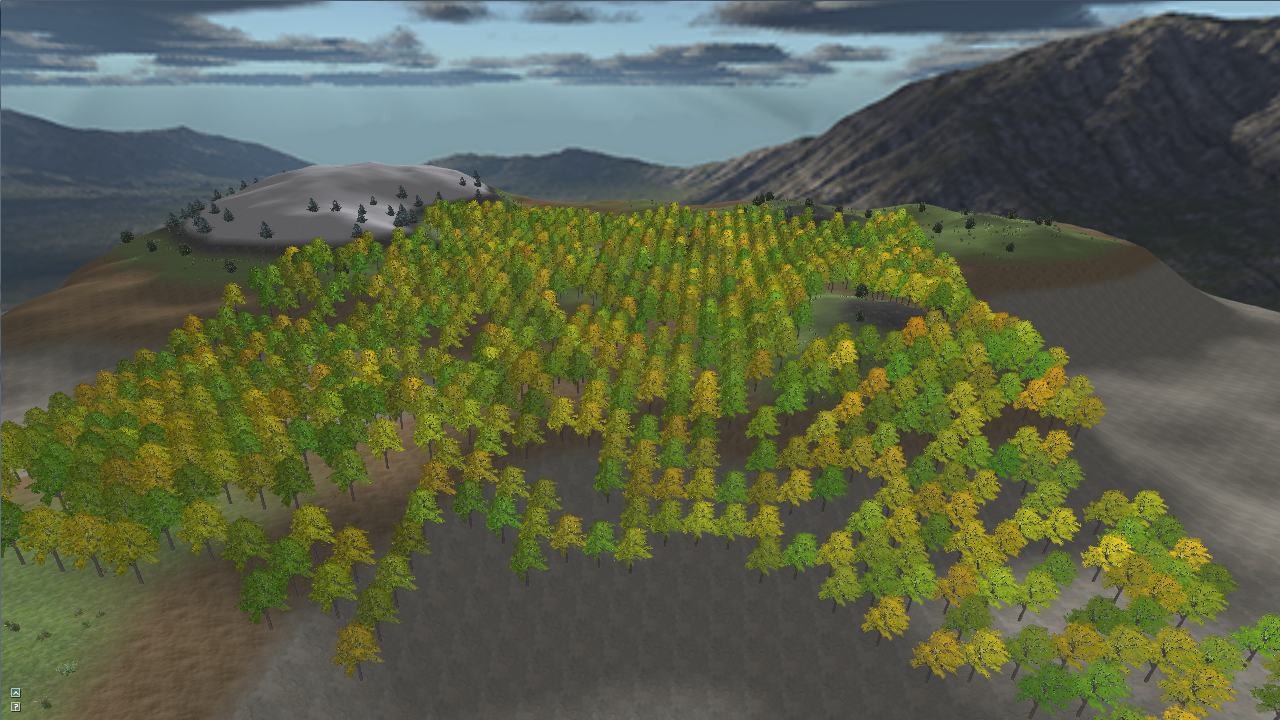
\includegraphics[width=0.3\textwidth]{./testing/LOD1only1000.png}&
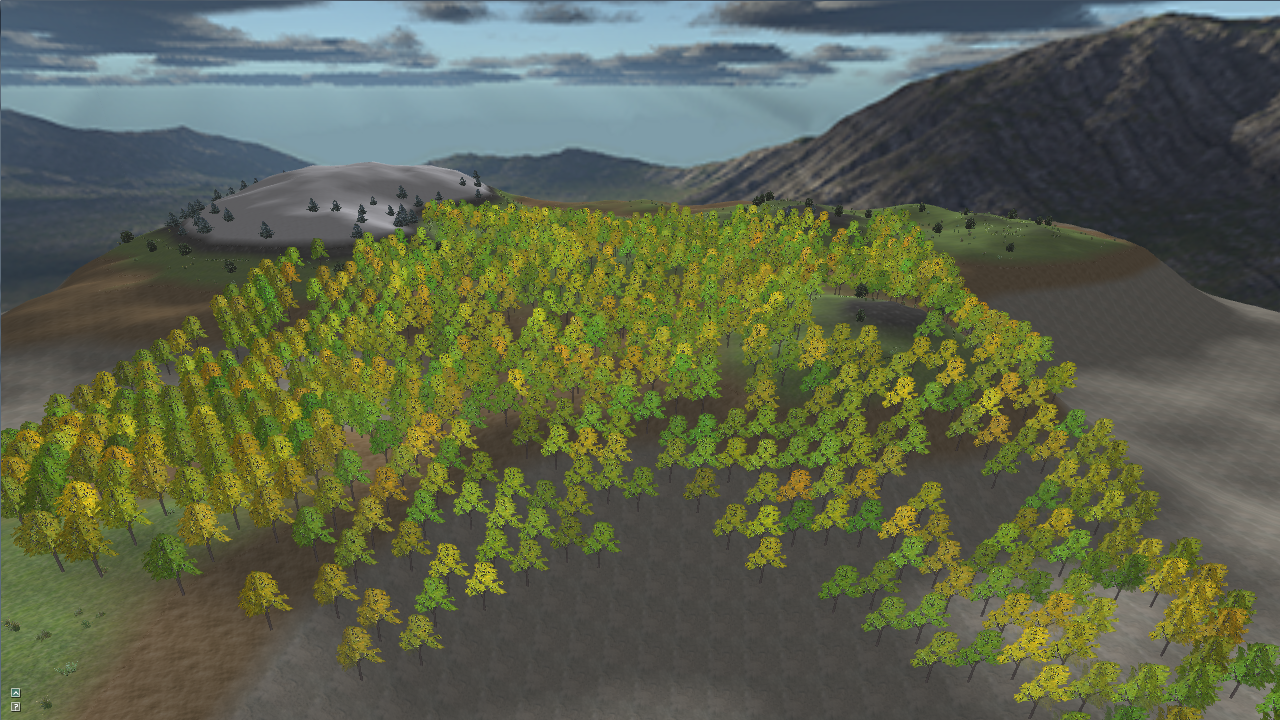
\includegraphics[width=0.3\textwidth]{./testing/LOD2only1000.png}
\\
(a)&(b)&(c)
\end{array}$
\end{center}
\caption[Náhledy testovací scény]%
{Náhledy z testování, scéna FOREST s 1000 instancemi , (a) LOD0,  (b) LOD1, (c) LOD2, 0\label{fig:testONLY}
}
\end{figure}

Následující tabuka uvádí hodnoty zobrazovacích časů naměřené pro různý počet instancí při zobrazování bez multisamplingu:
\begin{table}[!hbt]
\catcode`\-=12
\centering
\begin{tabular}{|r | c | c | l } 
\cline{1-3}
\#instancí & LOD0 (ms)& LOD1 (ms)& \\
\hline
\hline
10	&	2,98	&	3,71	& 	\multirow{3}{*}{scéna SMALL FOREST}\\
25	&	7,37		&	8,96	&	 \\
50	&	13,71	&	16,89	&	 \\
\hline
100	& 	20,25	&	6,54	&	\multirow{4}{*}{scéna FOREST}\\
250	& 	48,15	&	15,59	&\\
500	& 	94,73 	& 	30,36	&\\
1000 & 	188,96 	& 	57,16	&\\
\cline{1-3}
\end{tabular}
\caption{Porovnání LOD0 a LOD1, bez multisamplingu\label{table:lod01-1MS}}
\end{table}

A stejný test při vykreslování s multisamplingem (4 vzorky na pixel)

\begin{table}[!hbt]
\catcode`\-=12
\centering
\begin{tabular}{|r | c | c | l } 
\cline{1-3}
\#instancí & LOD0 (ms)& LOD1 (ms)& \\ [0.5ex] 
\hline
\hline
10	&	3,72	&	4,26	& 	\multirow{3}{*}{scéna SMALL FOREST}\\
25	&	8,32	&	9,48	&	 \\
50	&	15,94	&	16,5	&	 \\
\hline
100	& 	19,34	&	6,04	&	\multirow{4}{*}{scéna FOREST}\\
250	& 	47,5		&	14,36	&\\
500	& 	94,2 	& 	28,58	&\\
1000 & 	188,3 	& 	55,87	&\\
\cline{1-3}
\end{tabular}
\caption{Porovnání LOD0 a LOD1, 4x multisampling\label{table:lod01-4MS}}
\end{table}
 Jak se ukázalo, zpomalení způsobené zpracováváním více vzorků je takřka neznatelné. Potvrdil se i předpoklad, že rychlost zobrazování LOD0 závisí především na počtu zpracovávaných vrcholů (a tedy na počtu stromů), zatímco doba potřebná k vykreslení LOD1 závisí především na počtu fragmentů, do kterých je kresleno. Zatímco zobrazovací čas LOD0 s přibývajícími instancemi roste a je víceméně jedno, jak je scéna uspořádána, hraje pro LOD1 uspořádání scény důležitou roli, neboť {\bf zobrazení 50 instancí ve scéně SMALL FOREST trvá déle než zobrazení pětinásobného počtu (250) instancí ve scéně FOREST}. Záleží na výsledném pokrytí obrazu pixely instancí LOD1.
 Podstatné je ovšem zjištění, že pro malé scény je efektivnější využít LOD0, zatímco pro pohledy na rozsáhlé scény se již projevují přednosti a efektivita LOD1, které je pro 1000 instancí v testovaných scénách zhruba {\bf 3\texttimes efektivnější}. Jak se navíc ukázalo, je velice zásadní rozdíl při pohledu na instance LOD0 a LOD1 z větší vzdálenosti. Instance zobrazované v LOD0 ztratí listy a stanou se tak těžko použitelnými (viz porovnání na obr. \ref{fig:testQuality}). Tento jev souvisí s použitím částečně průhledných textur pro zobrazení jednotlivých listů. Při pohledu z dálky je taková textura vzorkována tak nešťastně, že se stává kompletně průhlednou. Naproti tomu, instance LOD1 si zachovávají svůj vzhled a co se týče kvality tak převyšují pro pohledy z dálky instance LOD0.

\begin{figure}[!hbt]
\begin{tabular}{r l}
LOD0: & 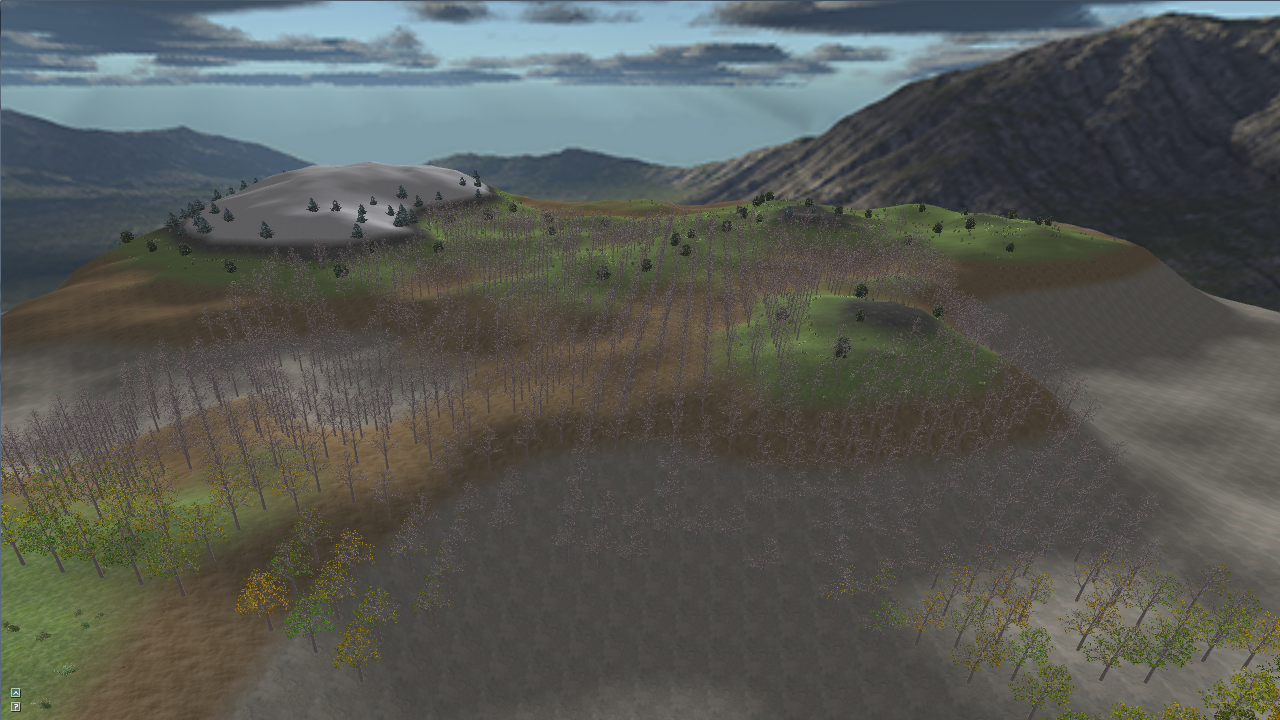
\includegraphics[width=0.8\textwidth]{./testing/LOD0only1000.png}\\
LOD1: & 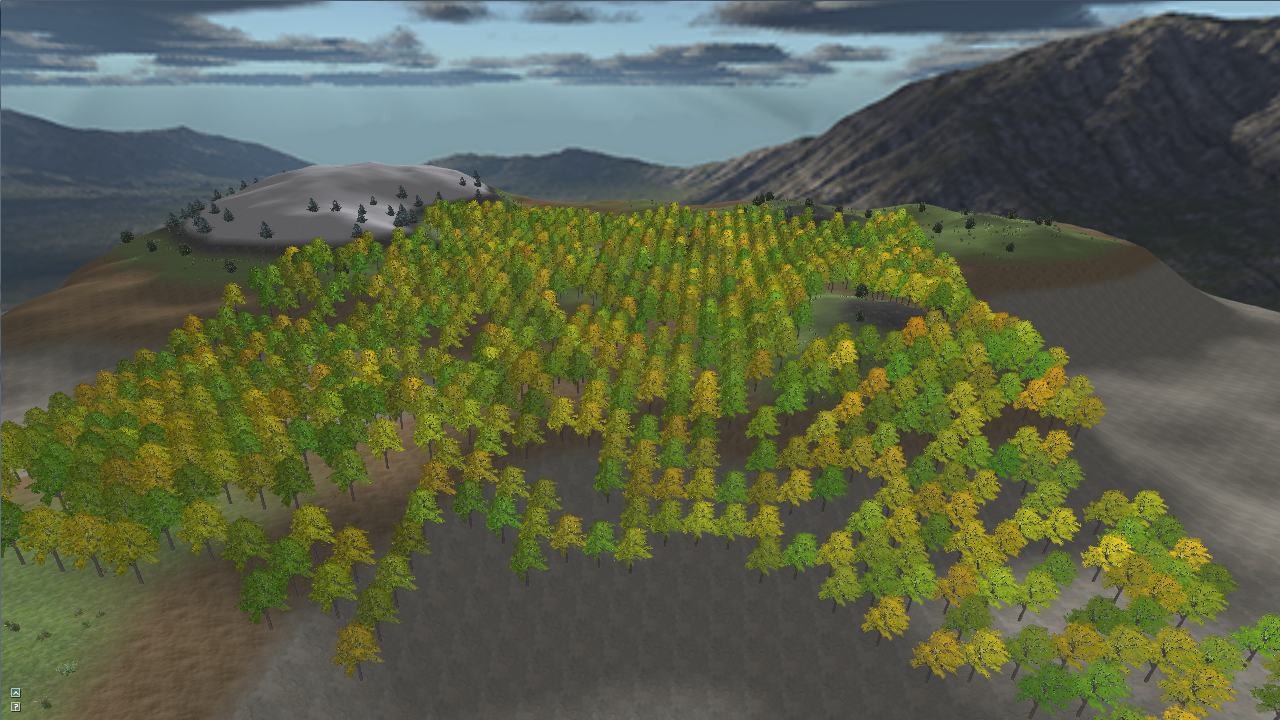
\includegraphics[width=0.8\textwidth]{./testing/LOD1only1000.png}\\
\end{tabular}
\caption[Náhledy testovací scény FOREST]%
{Náhledy z testování, scéna FOREST s 1000 instancemi, porovnání výsledné kvality \label{fig:testQuality}
}
\end{figure}

%%%%%%%%%%%%%%%%%%%%%%%%%%%%%%%%%%%%%
%	Fragmenty vs čas, 1 strom různé vzdálenosti
%
Silnou závislostí zobrazovacího času na počtu fragmentů se zabývá následující test. Je vytvořena scéna s jedinou instancí v počátku. Následně je měřen zobrazovací čas pro pohledy z různých vzdáleností. Využívá se vlastností perspektivní projekce, kdy vzdálenější objekty se jeví menší - a tedy jsou vykreslovány do menšího počtu fragmentů. Měření probíhalo bez multisamplingu a počet vykreslovaných fragmentů byl zaznamenáván pomocí Query Object čítače zpracovávaných fragmentů \lineCode{GL\_SAMPLES\_PASSED}. Jednotlivé pohledy na strom zachycuje sada obrázků~\ref{fig:testFRAG}. 
\begin{figure}[!hbt]
\begin{center}
$\begin{array}{ccccc}
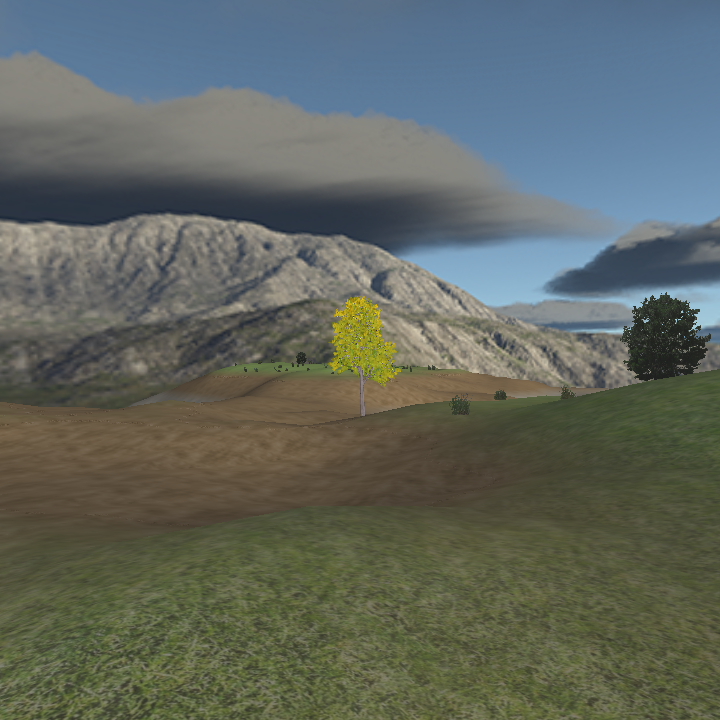
\includegraphics[width=0.17\textwidth]{./testing/LOD1-d50.png}&
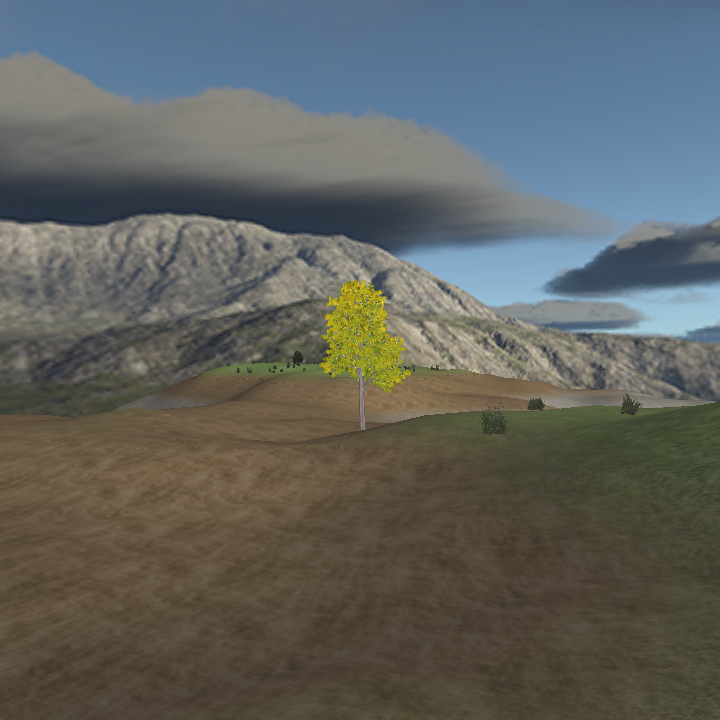
\includegraphics[width=0.17\textwidth]{./testing/LOD1-d40.png}&
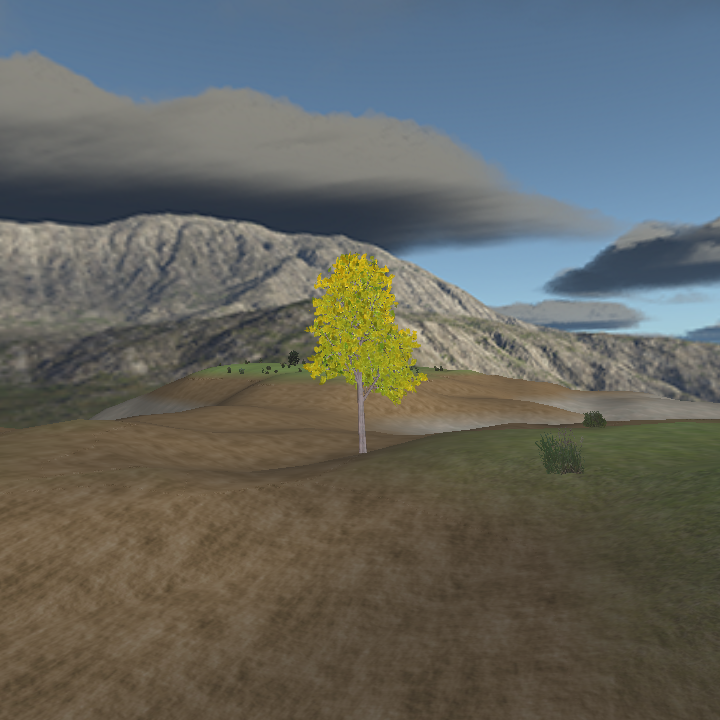
\includegraphics[width=0.17\textwidth]{./testing/LOD1-d30.png}&
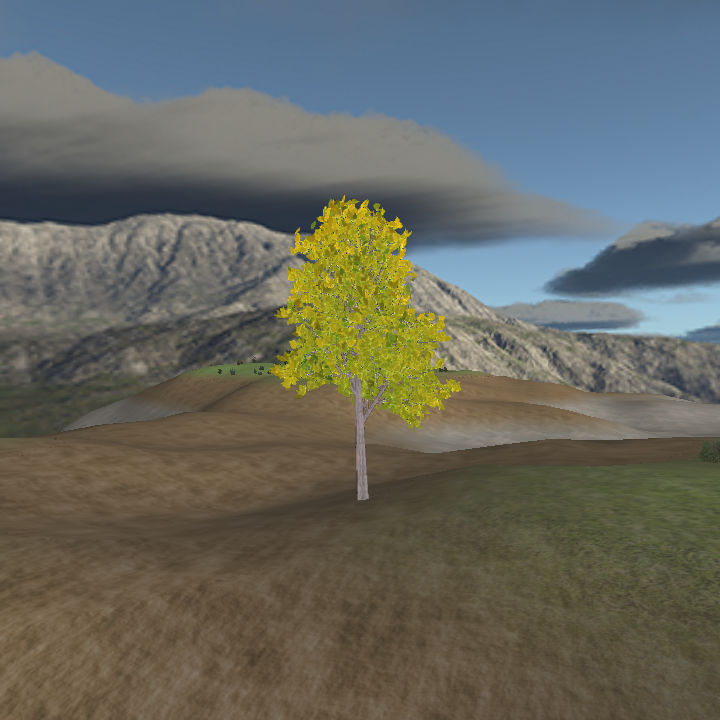
\includegraphics[width=0.17\textwidth]{./testing/LOD1-d20.png}&
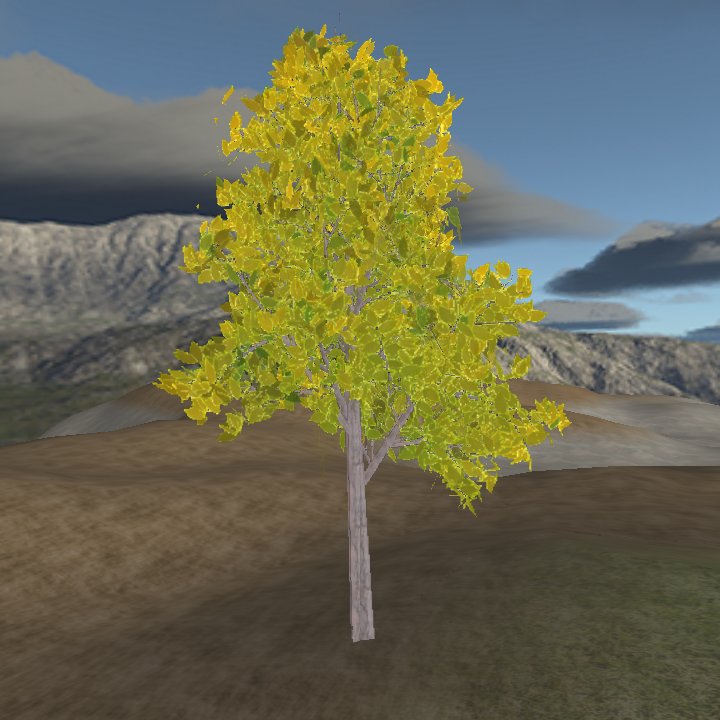
\includegraphics[width=0.17\textwidth]{./testing/LOD1-d10.png}
\\
(a)&(b)&(c)&(d)&(e)
\end{array}$
\end{center}
\caption[Náhledy testovací scény]%
{Náhledy z testování, scéna FRAGMENTS, (a) vzdálenost 50,  (b) vzdálenost 40, (c) vzdálenost 30, (d) vzdálenost 20, (e) vzdálenost 10\label{fig:testFRAG}
}
\end{figure}

Následující tabulka a grafy zprostředkovávají naměřené hodnoty pro vzdálenosti 10, 20, 30, 40 a 50 jednotek (velikost stromu je 10 jednotek).

\begin{table}[!hbt]
\centering
\begin{tabular}{|r | c | c | c | c | c | c |} 

\hline 
& \multicolumn{3}{c|}{LOD0}& \multicolumn{3}{c|}{LOD1}\\
vzdálenost & \# fragmentů & fps & čas (ms) & \# fragmentů & fps & čas (ms)\\
\hline
50		&4226		&1391,3		&0,71875	&6734		&1693,29	&0,59	\\
40		&7662		&1268,64	&0,78825	&10537		&1538,84	&0,65	\\
30		&15379		&1183,22	&0,84515	&18886		&1263,75	&0,79	\\
20		&39297		&1018,22	&0,98211	&43139		&928,04		&1,08	\\
10		&185531		&665,14		&1,50345	&180614		&389,14		&2,57	\\
\hline 
\end{tabular}
\caption{Závislost zobrazovacího času na počtu fragmentů.\label{table:lod01-fragtime}}
\end{table}

\begin{figure}[!hbt]
\begin{center}
$\begin{array}{cc}
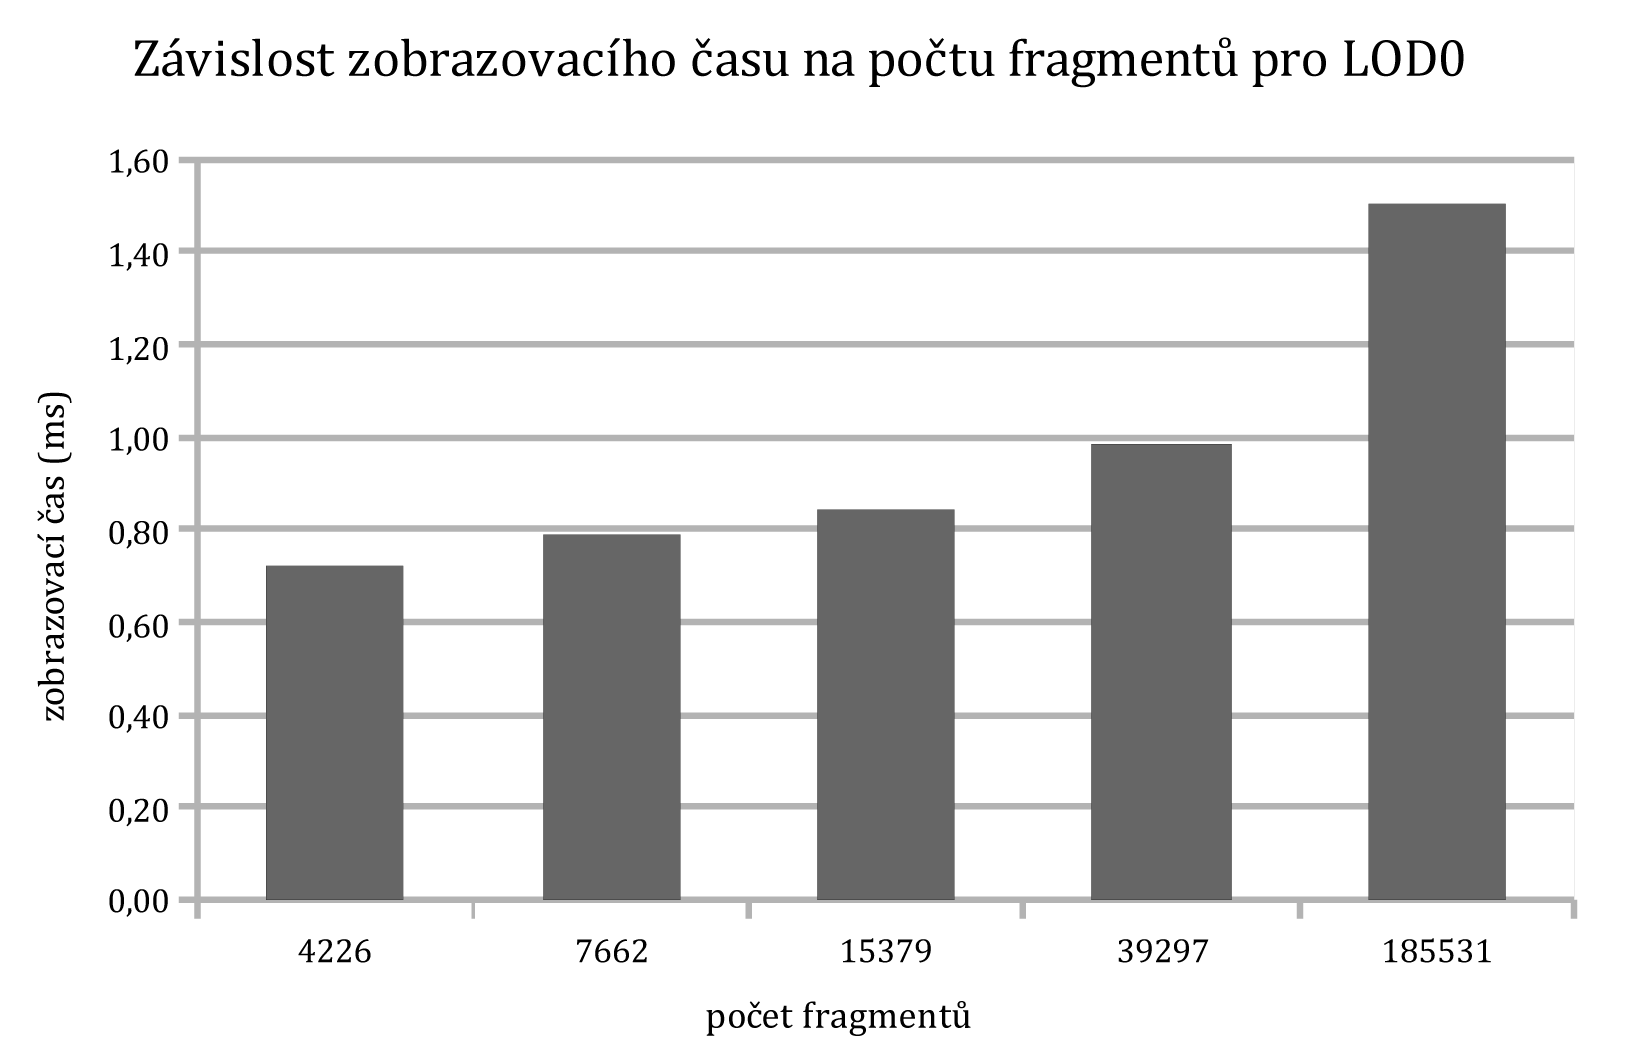
\includegraphics[width=0.45\textwidth]{./graphs/fragLOD0.png}&
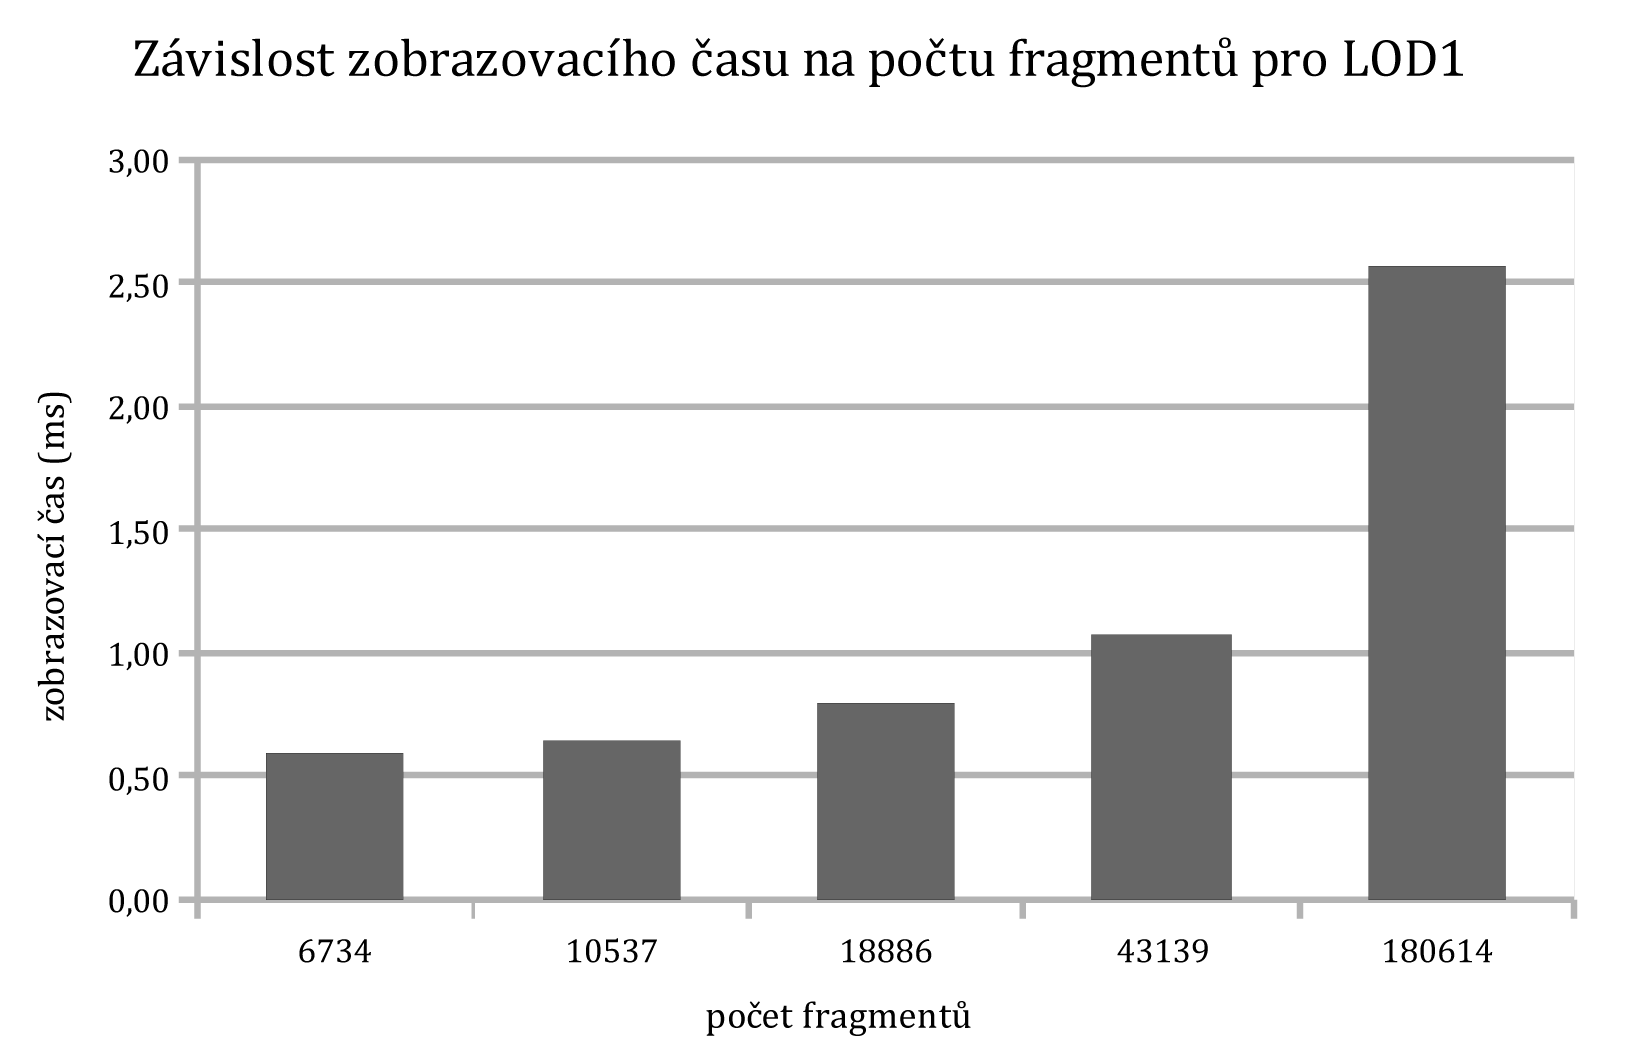
\includegraphics[width=0.45\textwidth]{./graphs/fragLOD1.png}
\\
(a)&(b)
\end{array}$
\end{center}
\caption[Grafy závislosti zobrazovacího času na počtu fragmentů]%
{Grafy závislosti zobrazovacího času na počtu fragmentů\label{fig:testFRAG}
}
\end{figure}

Vzájemná souvislost je pak dobře patrná z grafu na obr.~\ref{fig:testFRAG01}
\begin{figure}[!hbt]
\begin{center}
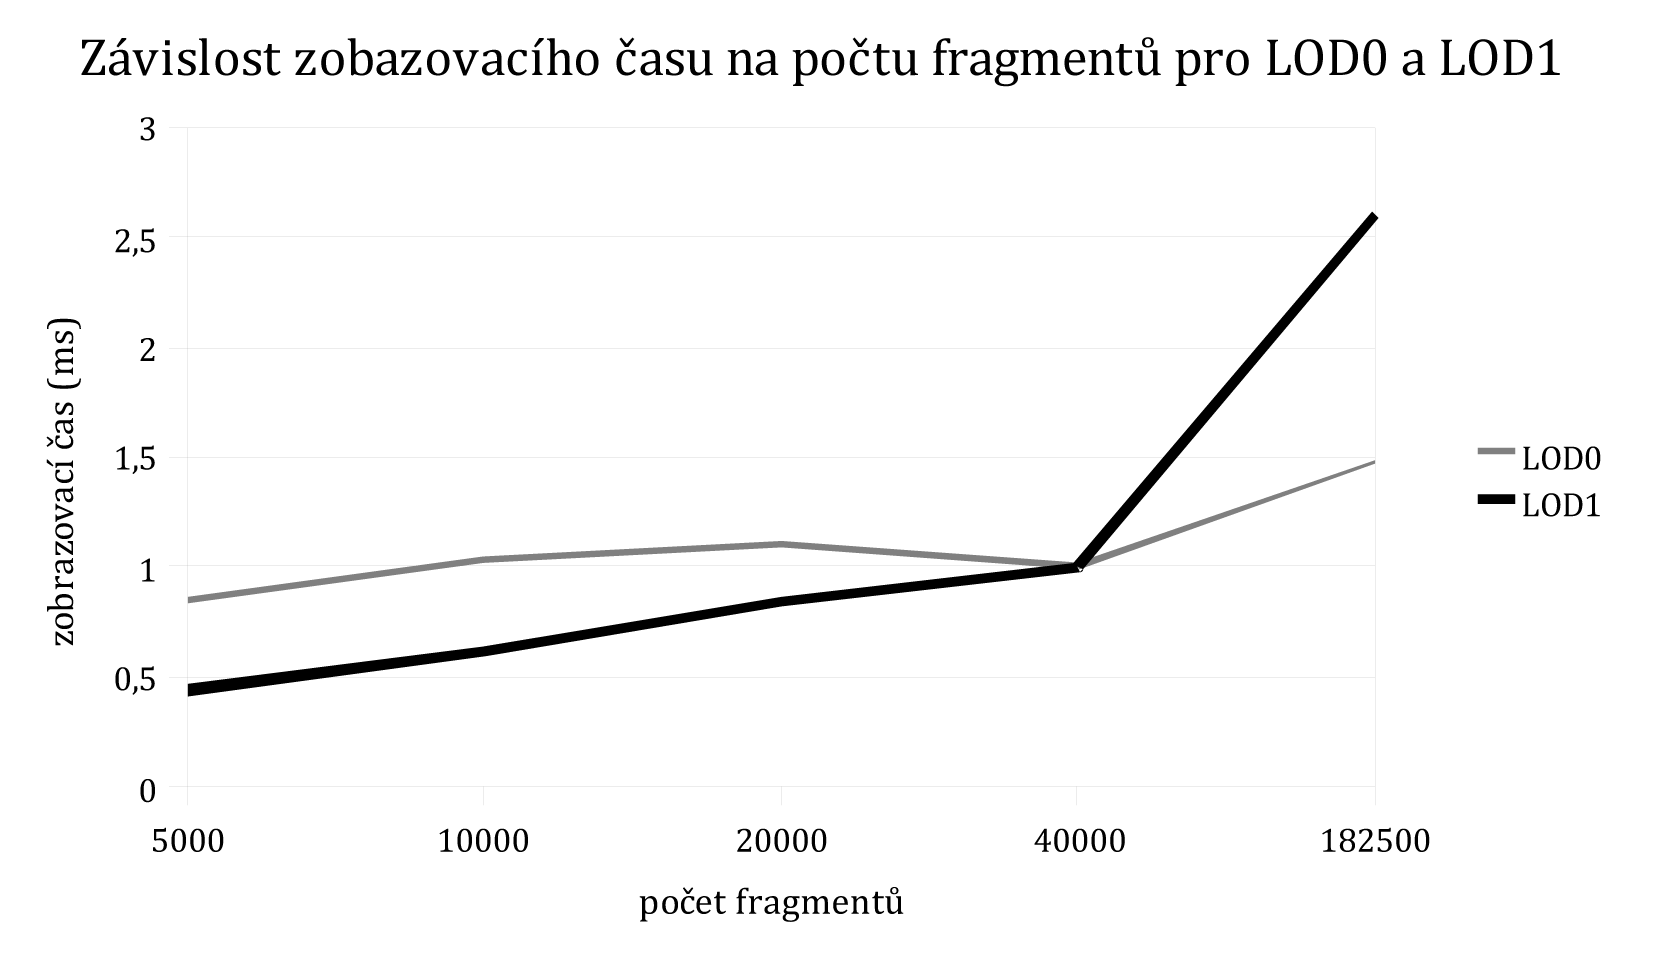
\includegraphics[width=0.75\textwidth]{./graphs/fragLOD01.png}
\end{center}
\caption[Graf závislosti zobrazovacího času na počtu fragmentů pro LOD0 a LOD1]%
{Graf závislosti zobrazovacího času na počtu fragmentů pro LOD0 a LOD1.\label{fig:testFRAG01}
}
\end{figure}

Je dobře patrné, že zatímco pro LOD0 je závislost na počtu fragmentů relativně nízká, pro LOD1 představuje silnou závislost. Pokud počet zpracovávaných fragmentů přesáhne hranici 40000, pak je zobrazování LOD1 časově náročnější než zobrazování LOD0.

%%%%%%%%%%%%%%%%%%%%%%%%%%%%%%%%%%%%%
%	Podil ruznych LOD na vyslednem case
%

Podíl jednotlivých LOD na výsledném zobrazovacím čase se snaží odhalit následující test. Scéna je zafixována (50 instancí stromů), jsou zafixované i vzdálenosti, ve kterých dochází k přechodu mezi LOD (viz obr.~\ref{fig:testCONTR}). Poté je scéna zobrazena nejprve bez stromů. Poté jsou zobrazeny pouze stromy v LOD0, následně jsou zobrazeny stromy v LOD1 a nakonec i v LOD2. 
\begin{figure}[!hbt]
\begin{center}
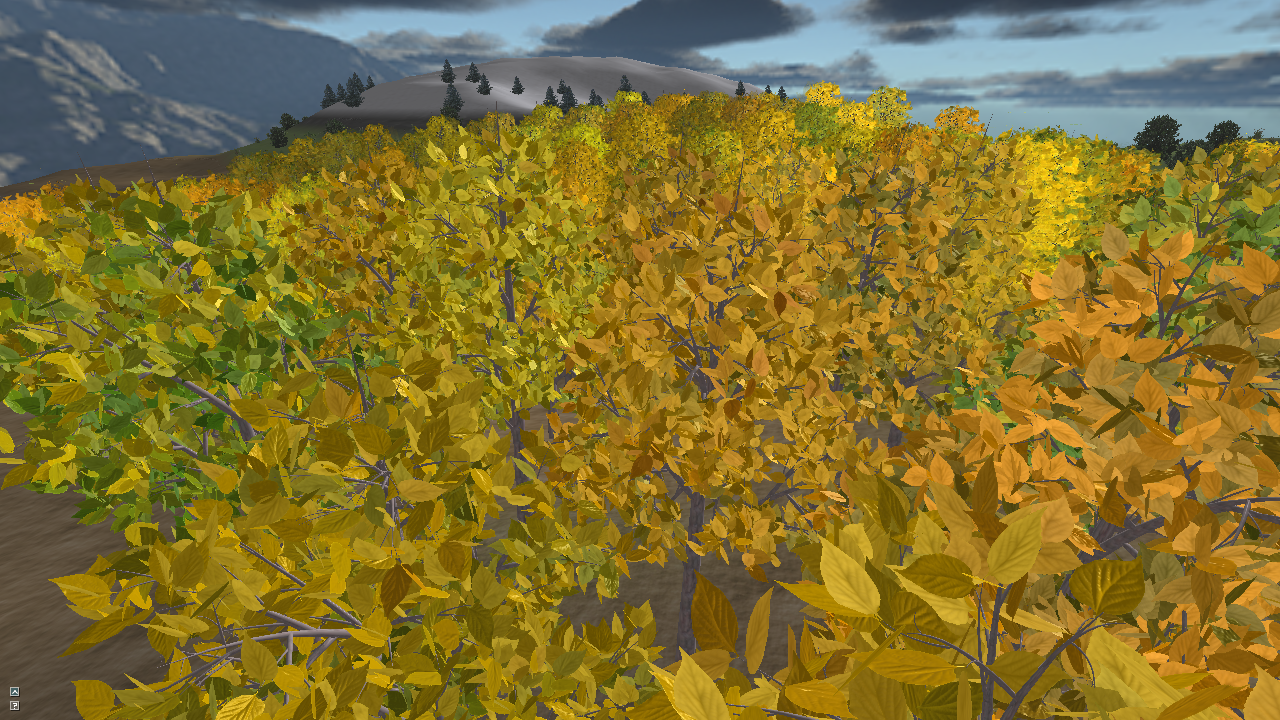
\includegraphics[width=0.5\textwidth]{./testing/on-offLOD2.png}
\end{center}
\caption[Náhled testovací scény podílu LOD na zobr. čase]%
{Náhled testovací scény podílu LOD na zobr. čase. \label{fig:testCONTR}
}
\end{figure}

\pagebreak
Výsledky měřená zaznamenává tabulka~\ref{table:lod012-contribs} a graf~\ref{gr:testCONTR}:

\begin{table}[!hbt]
\centering
\begin{tabular}{|r | c | c | c | c |} 
\hline 
 & fps & čas (ms) & rozdíl časů & \% \\
\hline
bez stromů		&2384,76	&0,42	&0,42	&1,46\\
LOD0			&112,64		&8,88	&8,46	&29,43\\
+LOD1			&36,7		&27,25	&18,37	&63,92\\
+LOD2			&34,79		&28,74	&1,49	&5,19\\
[1ex] 
\hline 
\end{tabular}
\caption{Podíly jednotlivých LOD na výsledném čase zobrazení\label{table:lod012-contribs}}
\end{table}

\begin{figure}[!hbt]
\begin{center}
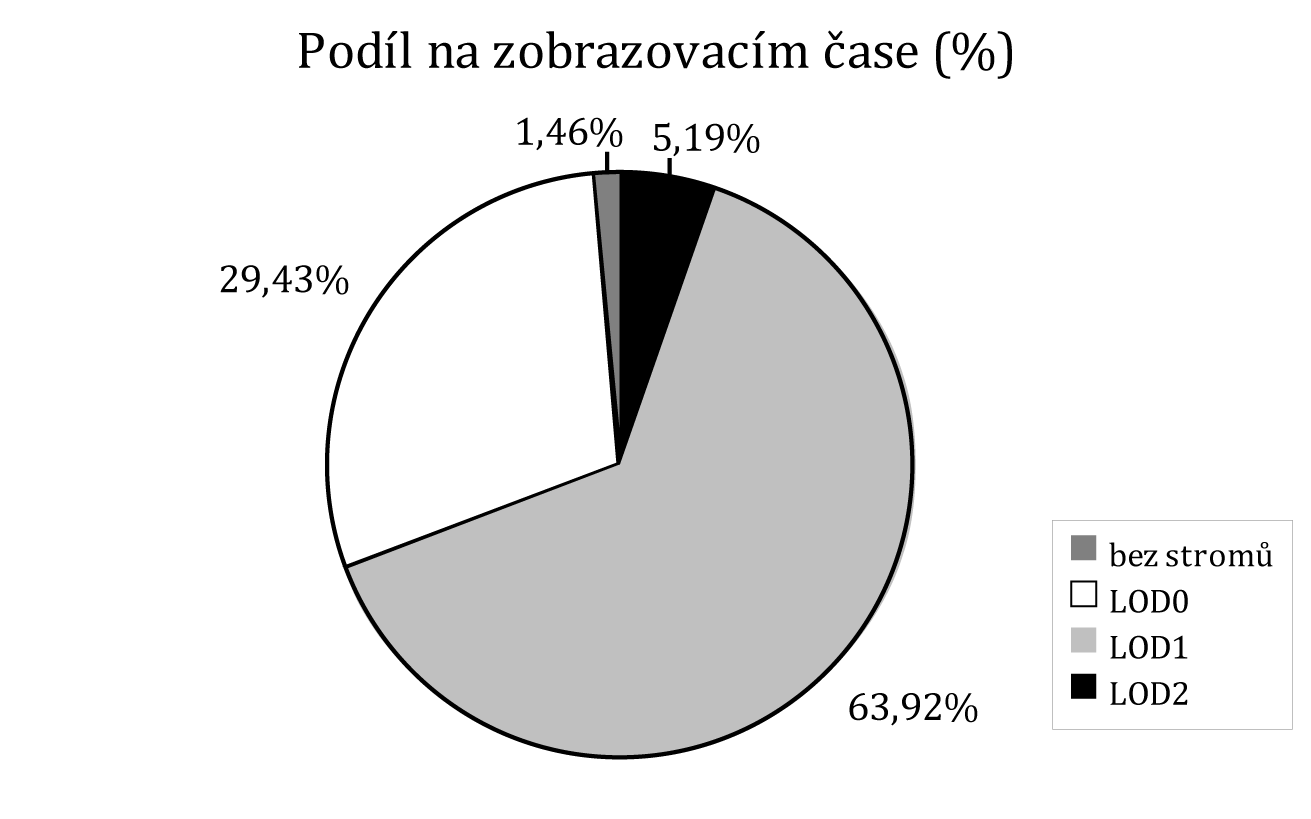
\includegraphics[width=0.6\textwidth]{./graphs/LODsContrib.png}
\end{center}
\caption[Graf podílů jednotlivých LOD na zobrazovacím čase]%
{Graf podílů jednotlivých LOD na zobrazovacím čase\label{gr:testCONTR}
}
\end{figure}

Je jasně patrné, že pro tuto scénu je časově nejnáročnější vykreslování instancí v LOD2, které z celkové doby 28,74 ms zabere více než polovinu (18,37 ms). 


%%%%%%%%%%%%%%%%%%%%%%%%%%%%%%%%%%%%%
%	Ruzne urovne animace
%

Další měření se týká toho, jak podrobnost animace LOD1 a LOD2 ovlivňuje časové nároky. Pro fixní scénu s různým počtem instancí stromů byl měřen zobrazovací čas pro různě podrobné animace. Byla změřena statická verze bez animace a následně byly přidávány úrovně animací. Nejprve pouze pohyb celého stromu (kmene), poté se přidaly i větve 1. úrovně. Nakonec, aby byla animace kompletní, byla měřena i plná verze LOD1 (resp. LOD2), včetně pohybu listů.
Výsledky měření obsahuje tabulka~\ref{table:lod12-anim}.
\begin{table}[!hbt]
\centering
\begin{tabular}{|l | c | c | c | c || c | c | c | c |} 
\hline 
		&\multicolumn{4}{c||}{LOD1}		&\multicolumn{4}{c|}{LOD2}\\	
		&\multicolumn{4}{c||}{\# instancí}	&\multicolumn{4}{c|}{\# instancí}\\
			&10		&25		&50		&100	&10		&25		&50		&100\\
\hline					
bez animace	&1,55	&3,39	&6,35	&11,31	&0,68	&1		&1,73	&2,68 \\
+ kmen		&2,64	&4,51	&8,14	&13,96	&1,35	&1,74	&3,07	&4,47\\
+ hlavní větve	&3,84	&7,73	&14,22	&23,53	&1,39	&3,06	&3,83	&4,75\\
+ listy			&4		&8,45	&16,91	&30,93	&1,79	&3,66	&4,14	&6,44\\
[1ex] 
\hline 
\end{tabular}
\caption{Vliv podrobnosti animace na zobrazovací čas. \label{table:lod12-anim}}
\end{table}

\pagebreak
Následující grafy (\ref{fig:testANIM1}~a~\ref{fig:testANIM2}) dávají tyto hodnoty do vzájemných souvislostí.
\begin{figure}[!hbt]
\begin{center}
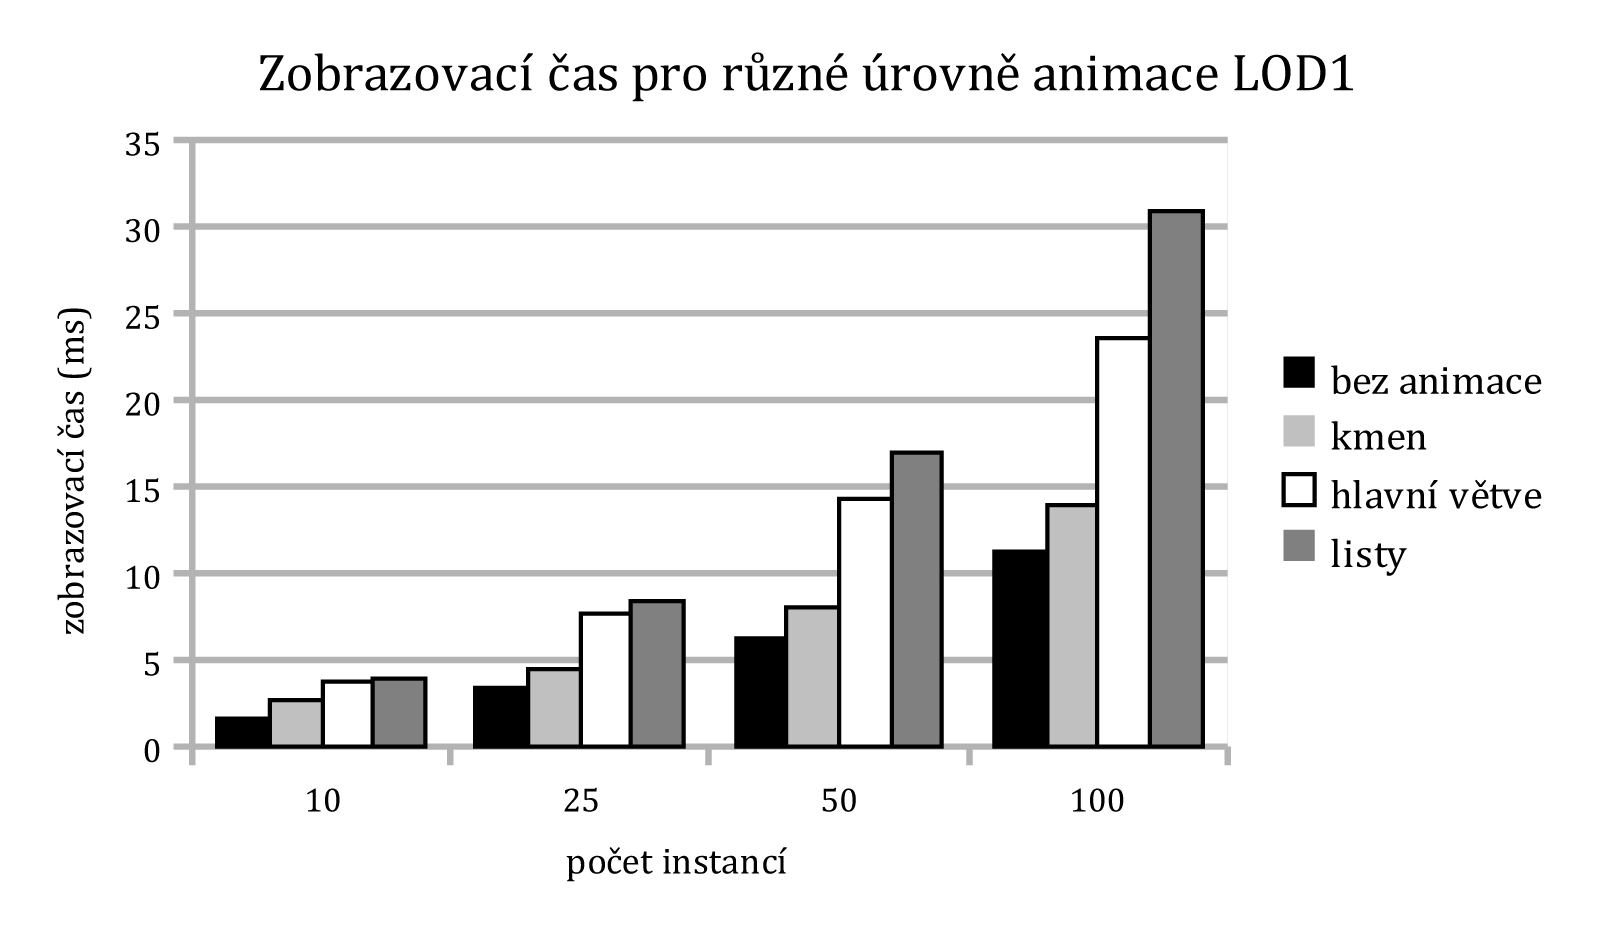
\includegraphics[width=0.75\textwidth]{./graphs/animLOD1.png}
\end{center}
\caption[Graf závislosti zobrazovacího času na podrobnosti animace LOD1]%
{Graf závislosti zobrazovacího času na podrobnosti animace LOD1.\label{fig:testANIM1}
}
\end{figure}
\begin{figure}[!hbt]
\begin{center}
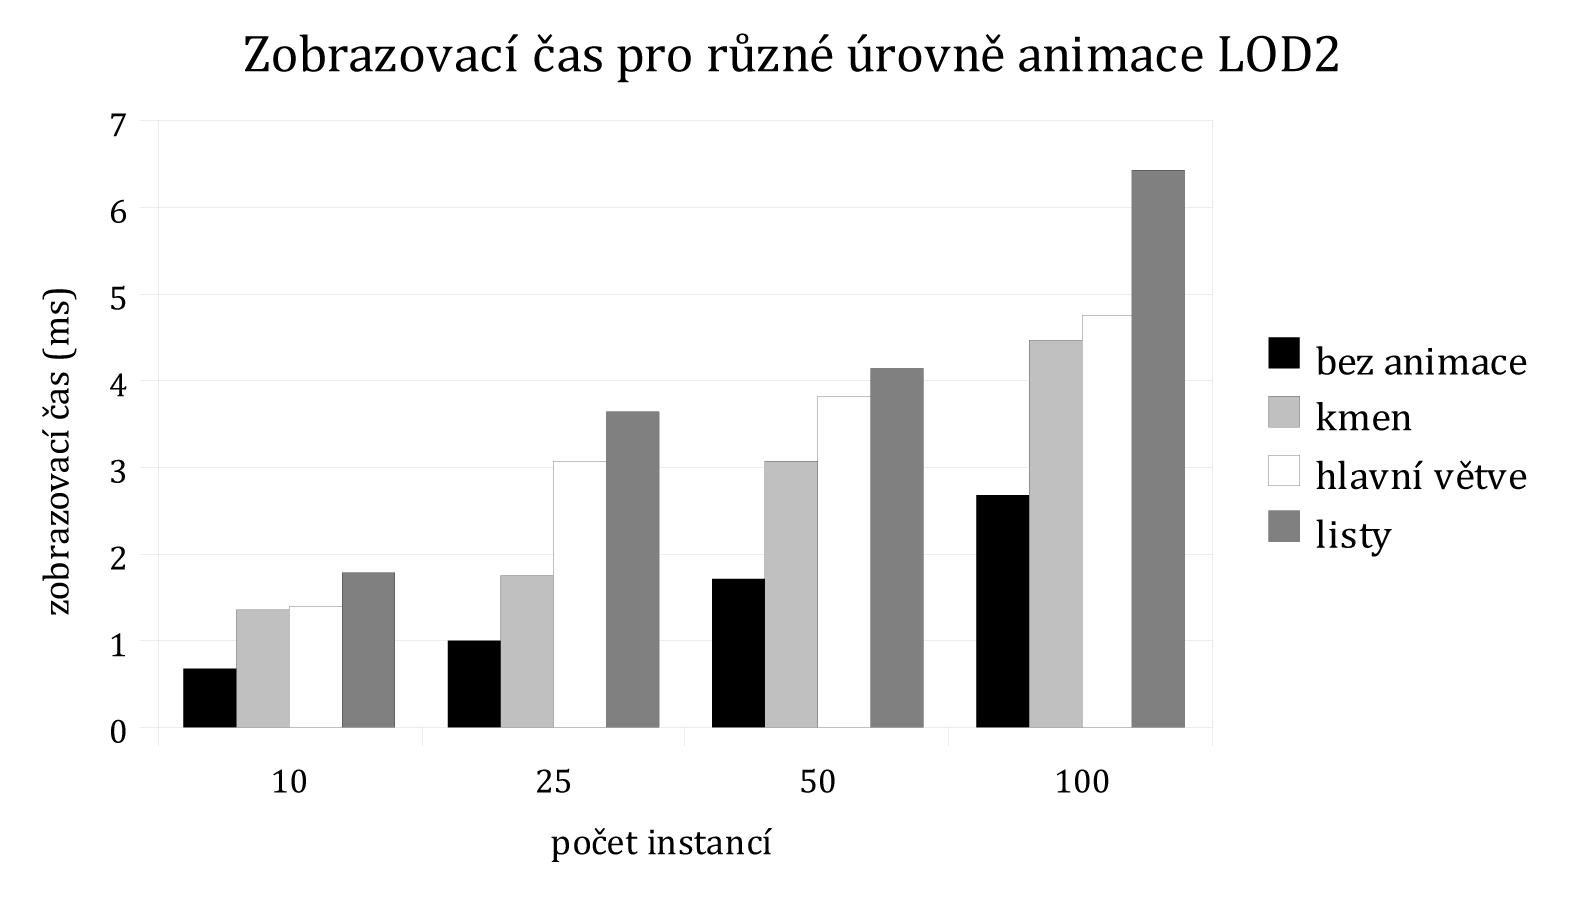
\includegraphics[width=0.75\textwidth]{./graphs/animLOD2.png}
\end{center}
\caption[Graf závislosti zobrazovacího času na podrobnosti animace LOD2]%
{Graf závislosti zobrazovacího času na podrobnosti animace LOD2.\label{fig:testANIM2}
}
\end{figure}

\pagebreak
%%%%%%%%%%%%%%%%%%%%%%%%%%%%%%%%%%%%%
%	Shadow mapping
%
Poslední test se zabývá tím, jaký vliv má rozlišení stínové mapy na zobrazovací čas pro různé instance. Měření probíhalo pouze s jedinou instancí, a fixovaným světelným zdrojem a scénou. Byly měřeny zobrazovací časy LOD0 a LOD1, přičemž LOD1 pro dva případy - s přepisem hloubky při zápisu do hloubkové textury a bez něj. Scéna byla vykreslována bez multisamplingu jak na obrazovku, tak do stínové mapy. Výsledky měření lze vyčíst z tabulky ~\ref{table:lod01-shadow}:
\begin{table}[!hbt]
\centering
\begin{tabular}{|r | c | c | c |} 
\hline 
&\multicolumn{3}{c|}{zobrazovací čas (ms)}\\
rozlišení stínové mapy			&LOD0		&LOD1 (přepis hloubky)	&LOD1 (bez přepisu)\\
\hline					
512 $\times$ 512	&2,26	&3,21	&3,28 \\
1024 $\times$ 1024	&2,44	&3,08	&3,02\\ 
2048 $\times$ 2048	&2,75	&5,98	&5,74\\
[1ex] 
\hline 
\end{tabular}
\label{table:lod01-shadow}
\caption{Vliv rozlišení stínové mapy na zobrazovací čas}
\end{table}

V zásadě se potvrdilo, že s rostoucím rozlišením se snižuje i rychlost vykreslování. Pro LOD1 je však zpomalení znatelnější. Rozdíl mezi postupem, kdy se přepisuje hloubka zapisovaná do stínové mapy, se pro danou scénu skoro neprojevil. Zajímavé ovšem je, že LOD1 se vykresluje rychleji při použití stínové mapy s rozlišením 1024\texttimes1024 px než při rozlišení 512\texttimes512 px. Toto chování lze zřejmě přičíst na vrub rozdílné optimalizaci ze stany GPU při použití různých rozlišení. Odhalení konkrétní příčiny by vyžadovalo další studium tohoto jevu.

V rámci testování byla zachycena z okna aplikace videa, která dokazují, že systém pracuje na testovací sestavě v reálném čase. Tato videa lze nalézt na přiloženém datovém nosiči.